%---------- Inleiding ---------------------------------------------------------

% TODO: Is dit voorstel gebaseerd op een paper van Research Methods die je
% vorig jaar hebt ingediend? Heb je daarbij eventueel samengewerkt met een
% andere student?
% Zo ja, haal dan de tekst hieronder uit commentaar en pas aan.

%\paragraph{Opmerking}

% Dit voorstel is gebaseerd op het onderzoeksvoorstel dat werd geschreven in het
% kader van het vak Research Methods dat ik (vorig/dit) academiejaar heb
% uitgewerkt (met medesturent VOORNAAM NAAM als mede-auteur).
% 
\section{Inleiding}%
\label{sec:inleiding}
Voor deze bachelorproef werk ik samen met Tracked, een compentence center binnen de Cronos groep gespecialiseerd in traceerbaarheid van de toeleveringsketen in de industrie, en gaan we aan de slag met traceringsdata van ArcelorMittal Gent.

Binnen ArcelorMittal Gent bestaan er veel verschillende processen die verspreid zijn over meerdere afdelingen.
Hierbij bevat elke afdeling een deel van het proces om van grondstof tot een afgewerkt product te komen. 
Tussen elke afdeling bevindt zich een deel van de toeleveringsketen, waarbij het resultaat van de ene afdeling het beginpunt is voor de volgende afdeling.
Dit zorgt ervoor dat iedere stap zijn invloed heeft op de kwaliteit van het eindresultaat.

Elke afdeling is opgebouwd rond een specifiek proces, zoals de hoogoven die ruwe grondstoffen omzet in ruw ijzer en de staalfabriek die ruw ijzer in staal verandert.
Omdat deze afdelingen zeer specifieke processen hebben, hebben ze ook zeer specifieke behoeften en datamodellen.
Dit maakt analyse of onderzoek over afdelingen heen zeer complex en tijdsrovend.

De scope van deze bachelorproef is tweedelig, waarbij deel één eruit bestaat om samen met Tracked vanuit een gestandariseerd datamodel die zichtbaarheid events bijhoudt om te zetten naar een grafiekmodel.
Deel twee bouwt verder voort op dit grafiekmodel om dan een LLM (large language model) te trainen die eenvoudig informatie eruit kan halen en teruggeven.

De centrale vraag die hier gesteld wordt is: ``Hoe we efficiënt en snel grafiekmodellering kunnen toepassen om een LLM te ontwikkelen die in staat is om het waar, wanneer, wat en hoe van gebeurtenissen binnen een proces vast te stellen, ter ondersteuning van klachtenafhandeling bij productfouten.``
%---------- Stand van zaken ---------------------------------------------------
\section{Literatuurstudie}%
\label{sec:literatuurstudie}

\subsection{Cosmos DB}%
Cosmos DB is een NoSQL-database van Microsoft. Het biedt een lage latentie, multi-query-API die eenvoudig grote hoeveelheden data kan verwerken en heeft een grote beschikbaarheid zegt~\textcite{Put2020}, wat zeer belangrijk is in ons project.
Daarnaast is CosmosDB horizontaal schaalbaar, wat betekent dat we op hoogtepunten tot een miljoen lees- en schrijfaanvragen kunnen verwerken door het benodigde aantal servers toe te voegen.
De hoge beschikbaarheid wordt gegarandeerd door replicatie, waardoor we snel kunnen overschakelen als er een probleem is in onze database.

\subsection{Grafiek modellering}
In een grafiekdatabase slaan we gegevens op in de vorm van vertices (knopen) en edges (relaties), hierdoor kunnen we complexe verbanden leggen zoals in ons geval de productieprocessen.
Cosmos DB ondersteunt ook grafiekmodellering met behulp van Gremlin API. Gremlin is gebasseerd op Apache tinkerpop's Gremlin, dit is een krachtig grafiekverwerkingsframework waarbij we grote grafieken kunnen opslaan, modelleren en doorzoeken via gremlin traversal language \autocite{Microsoft2024}.
Dit gebeurt met een snelheid van milliseconden waardoor we een snelle verwerkingstijd zullen kunnen neerzetten.
Daarnaast is Gremlin ook schaalbaar en kan het consistentie level gekozen worden om een balans te vinden tussen consistentie, beschikbaarheid en latentie.
Binnen zo'n grafiek model hebben we vertices (of nodes) die een persoon, plaats of event beschrijven zoals in ons geval bijvoorbeeld een slab die wordt verplaatst van A naar B.

\subsubsection{Verschil transformatie en aggregatie}
Binnen ons project kunnen de bestaansvormen van producten veranderen. Zo hebben we transformatie, dit is een deel van het proces waarbij de verandering van het product onomkeerbaar is.
Daarnaast hebben we aggregatie waarbij we wel terug naar de oorspronkelijke vorm zouden kunnen gaan indien nodig.
In onze grafiekmodellering moeten we gebruik maken van tijdelijke edges om ook terug te kunnen kijken naar wat voor het transformatie- of aggregatieproces gebeurd is, om zo anomalieën terug te vinden \autocite{JaewookByun2020}.

\subsection{Retrieval Augmented Generation}
Om onze chatbot te optimaliseren gaan we gebruik maken van RAG.
Dit zorgt ervoor dat de antwoorden die de chatbot zal geven niet out-dated zijn en een geldige bron bevatten (zoals onze eigen data) \autocite{IBM2023}.
Binnen een LLM waarbij je RAG gebruikt zal de user een prompt geven, daarna gaat het LLM vragen aan RAG om alle bronnen (data) te geven over het gevraagde onderwerp.
Zodra hij jouw prompt samen heeft gevoegd met de data die erover beschikbaar is geeft hij een correct antwoord terug.
In ons geval kunnen we bijvoorbeeld vragen waar de container staal was op een bepaalde datum, en op dat moment vraagt het LLM aan RAG alle informatie over die container waarna hij een geschikt antwoord kan geven.
Deze methode wordt ook gebruikt in onder andere ChatGPT en andere LLM's om ervoor te zorgen dat je het model zelf niet herhaaldelijk moet trainen, maar een up-to-date dataset aan koppelt.
Kort gezegd is RAG een AI framework dat data gebruikt buiten zijn eigen getrainde data om te voorkomen dat je het model moet blijven updaten.
\subsubsection{RAG vs Finetuning}
Bij RAG gebruiken we een soort database waarbij het model up-to-date blijft en geldige bronnen gebruikt. Dit is voordelig in ons project omdat er dagelijks heel veel staal geproduceerd wordt en dus veel verschillende processen zijn.
Daarnaast hebben we finetuning waarbij we onze eigen stijl kunnen geven aan het model door bepaalde vakjargon toe te voegen of het model sneller te maken \autocite{IBM2024}.
Maar er moet wel zorgvuldig met finetuning omgegaan worden, want het kan snel veel rekenkracht vragen of zelfs voor overfitting zorgen waarbij de trainingsdata goed presteert, maar ongeziene data niet zegt \textcite{EASIIO2022}.
Een combinatie van deze 2 methodes zou in ons scenario ideaal zijn. Dit komt doordat ArcelorMittal veel vakjargon hanteert, zoals cokes en slabs. Hierdoor kunnen we ons model specialiseren. Daarnaast moet de data die we gebruiken specifiek en up-to-date zijn, zodat we altijd van elk moment op de hoogte blijven

\subsection{EPCIS}
Voor dit onderzoek moet alles voldoen aan de EPCIS (Electronic Product Code Information Services) waarden, dit zijn de wat, wanneer, waar, waarom en hoe. 
Deze waarden zijn ontwikkeld door GS1 om gegevens over beweging, status en verandering van een item in de toeleveringsketen (supply chain) vast te leggen en te delen binnen en buiten het bedrijf \autocite{Devins}.
``Met behulp van deze waarden kunnen we real-life objecten omzetten in elektronisch opgeslagen informatie, waarna we dit kunnen communiceren met eindgebruikers.`` zegt \textcite{Devins}.
Door deze normen toe te passen kunnen we de traceerbaarheid van het product per proces garanderen inclusief de gewenste parameters die opgeslagen worden in ons grafiekmodel zoals tijd (wanneer) en temperatuur (hoe) waar nodig.
\subsubsection{Waarom EPCIS?}
Huidige Legacy Systemen maken gebruik van ERP, POS, WMS,\dots Vaak lopen deze niet real-time wat nadelig is als we direct iets willen weten over een product en hoge beschikbaarheid verwachten \autocite{Vieweger}.
Doordat elk bedrijf eenzelfde norm gebruikt kunnen we dit schaalbaar houden en makkelijk uitbereiden.



% Hier beschrijf je de \emph{state-of-the-art} rondom je gekozen onderzoeksdomein, d.w.z.\ een inleidende, doorlopende tekst over het onderzoeksdomein van je bachelorproef. Je steunt daarbij heel sterk op de professionele \emph{vakliteratuur}, en niet zozeer op populariserende teksten voor een breed publiek. Wat is de huidige stand van zaken in dit domein, en wat zijn nog eventuele open vragen (die misschien de aanleiding waren tot je onderzoeksvraag!)?

% Je mag de titel van deze sectie ook aanpassen (literatuurstudie, stand van zaken, enz.). Zijn er al gelijkaardige onderzoeken gevoerd? Wat concluderen ze? Wat is het verschil met jouw onderzoek?

% Verwijs bij elke introductie van een term of bewering over het domein naar de vakliteratuur, bijvoorbeeld~\autocite{Hykes2013}! Denk zeker goed na welke werken je refereert en waarom.

% Draag zorg voor correcte literatuurverwijzingen! Een bronvermelding hoort thuis \emph{binnen} de zin waar je je op die bron baseert, dus niet er buiten! Maak meteen een verwijzing als je gebruik maakt van een bron. Doe dit dus \emph{niet} aan het einde van een lange paragraaf. Baseer nooit teveel aansluitende tekst op eenzelfde bron.

% Als je informatie over bronnen verzamelt in JabRef, zorg er dan voor dat alle nodige info aanwezig is om de bron terug te vinden (zoals uitvoerig besproken in de lessen Research Methods).

% Voor literatuurverwijzingen zijn er twee belangrijke commando's:
% \autocite{KEY} => (Auteur, jaartal) Gebruik dit als de naam van de auteur
%   geen onderdeel is van de zin.
% \textcite{KEY} => Auteur (jaartal)  Gebruik dit als de auteursnaam wel een
%   functie heeft in de zin (bv. ``Uit onderzoek door Doll & Hill (1954) bleek
%   ...'')

% Je mag deze sectie nog verder onderverdelen in subsecties als dit de structuur van de tekst kan verduidelijken.
\newpage
%---------- Methodologie ------------------------------------------------------
\section{Methodologie}%
\label{sec:methodologie}
Eerst en vooral gaan we aan de slag met een json bestand dat data bevat van ArcelorMittal waar events in opgeslagen staan.
Daarna zetten we dit om naar Cosmos DB (de door Tracked gebruikte database service) en kunnen we via Gremlin API werken om een grafiek op te zetten met tijdsgebonden edges. Dit dient ervoor om te zorgen dat we in tijd terug kunnen om de historiek op te vragen en te kijken waar, wanneer en hoe een proces gebeurd is.
Daardoor kunnen we achteraf bij onder andere klachtenafhandeling terug kijken in het grafiekmodel wat er mogelijks anders was of fout is gelopen.

Dit grafiekmodel moet ook voldoen aan de normen volgens EPCIS en schaalbaar zijn, daarom gaan we zorgen dat de gebruikte data binnen het grafiekmodel zoals een node een id krijgt in de plaats van een statische naam.
Daardoor kan Tracked in latere fases of andere business cases dezelfde technieken gebruiken zonder veel aanpassingen te moeten doen op grote schaal.

Zodra we een duidelijk grafiekmodel hebben waarmee we makkelijk in het verleden kunnen kijken, kunnen we dit trainen met copilot van microsoft.
Daarna gaan we op zoek naar de beste methode om dit te implementeren met onder andere hulp van de RAG methode en finetuning. Daarnaast gaan we ook nog op zoek naar een geschikt zoekalgoritme om zo snel mogelijk op de juiste data terecht te komen.
Daardoor kunnen we dan snel zoeken naar waar mogelijks anomalieën zijn in een proces door te vergelijken met andere batches die hetzelfde proces hebben doorlopen.
Als laatste kunnen we dan via copilot makkelijk een implementatie starten voor onder andere Microsoft Teams waarbij iemand van de klantenservice kan vragen wat er fout is gelopen en dat de chatbot zegt waar, wanneer en hoe er mogelijks een fout is geweest in het proces.


% - Eerste fase -> begrijpen wat tijdelijke transfereerbare graph techniek is. Werken met CosmosDB heeft grammling API embedded (apache gremlin (https://tinkerpop.apache.org/gremlin.html)). EPCIS Datamodel leren (events van AM transformeren naar Gremlin)
% - Tweede fase -> Aanleren copilot studio (microsoft) en hoe linken met graph en chatbot maken.

% Hier beschrijf je hoe je van plan bent het onderzoek te voeren. Welke onderzoekstechniek ga je toepassen om elk van je onderzoeksvragen te beantwoorden? Gebruik je hiervoor literatuurstudie, interviews met belanghebbenden (bv.~voor requirements-analyse), experimenten, simulaties, vergelijkende studie, risico-analyse, PoC, \ldots?

% Valt je onderwerp onder één van de typische soorten bachelorproeven die besproken zijn in de lessen Research Methods (bv.\ vergelijkende studie of risico-analyse)? Zorg er dan ook voor dat we duidelijk de verschillende stappen terug vinden die we verwachten in dit soort onderzoek!

% Vermijd onderzoekstechnieken die geen objectieve, meetbare resultaten kunnen opleveren. Enquêtes, bijvoorbeeld, zijn voor een bachelorproef informatica meestal \textbf{niet geschikt}. De antwoorden zijn eerder meningen dan feiten en in de praktijk blijkt het ook bijzonder moeilijk om voldoende respondenten te vinden. Studenten die een enquête willen voeren, hebben meestal ook geen goede definitie van de populatie, waardoor ook niet kan aangetoond worden dat eventuele resultaten representatief zijn.

% Uit dit onderdeel moet duidelijk naar voor komen dat je bachelorproef ook technisch voldoen\-de diepgang zal bevatten. Het zou niet kloppen als een bachelorproef informatica ook door bv.\ een student marketing zou kunnen uitgevoerd worden.

% Je beschrijft ook al welke tools (hardware, software, diensten, \ldots) je denkt hiervoor te gebruiken of te ontwikkelen.

% Probeer ook een tijdschatting te maken. Hoe lang zal je met elke fase van je onderzoek bezig zijn en wat zijn de concrete \emph{deliverables} in elke fase?

%---------- Verwachte resultaten ----------------------------------------------
\section{Verwacht resultaat, conclusie}%
\label{sec:verwachte_resultaten}
In dit onderzoek maken we startlaag aan een groter project waarbij het mogelijk is om uit te bereiden naar bijvoorbeeld een planningstool om de meest efficiënte route te zoeken.
Door deze chatbot verwachten we dat medewerkers van ArcelorMittal eenvoudig een vraag kan stellen en een antwoord kan krijgen op een korte tijd.
Zonder deze optie moeten ze elk deel van het bedrijf handmatig opbellen en vragen wat er gebeurd is, dat zijn zaken die zeer tijdsslopend zijn en veel geld kosten.
Er wordt gehoopt dat we een schaalbaar systeem kunnen opstellen en dit performant kunnen houden waardoor het gebruikt kan worden op nationaal en/of internationaal niveau.
Met de implementatie van dit systeem wordt er gestreefd naar de optimalisatie van klanttevredenheid en besparingen binnen een bedrijf, in dit geval ArcelorMittal Gent.
\begin{figure}[h!]
    \centering
    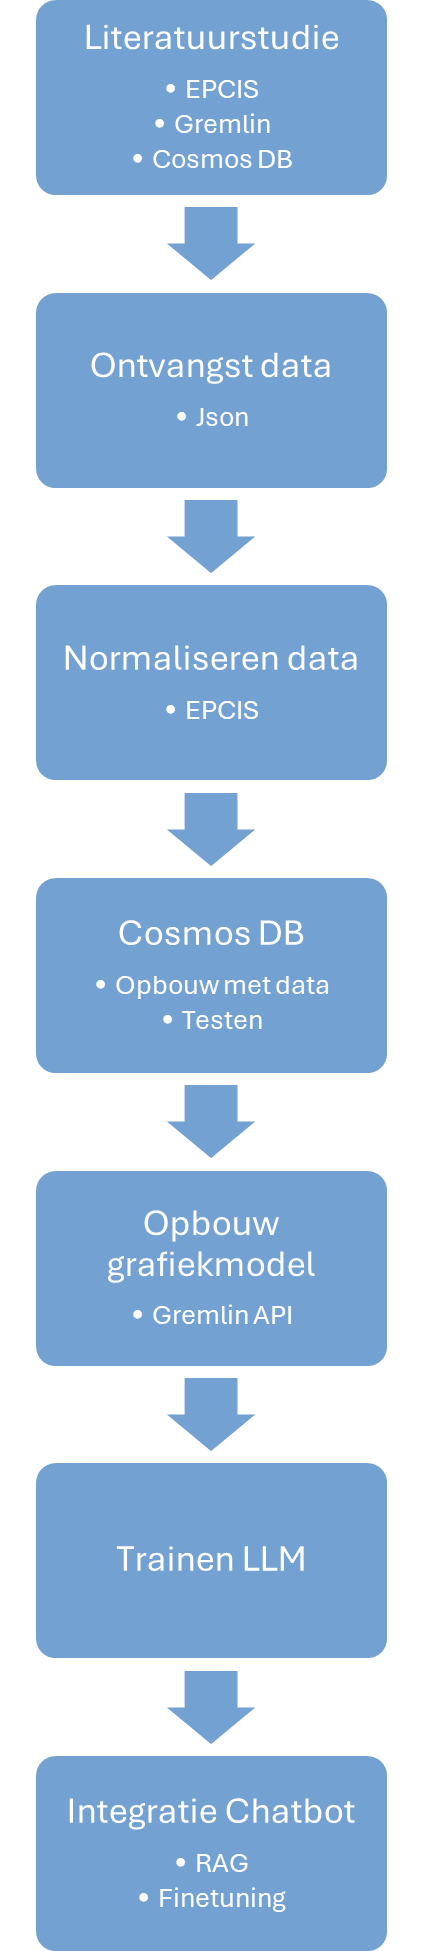
\includegraphics{../graphics/flowchart.png}
    \caption{\label{fig:chart}Flowchart}
\end{figure}
% - Kan een medewerken van ArcelorMittal op een eenvoudige manier een antwoord vinden op zijn vraag en wat is de tijdswints & geldbesparing dat ermee gepaard gaat.
% - Kunnen we op een bepaalde schaalgrootte de grafiek maken en performant houden
% BusinessUC -> Moet opgenomen worden in verwahte resultaat kost/besparing samenleggen.


% Hier beschrijf je welke resultaten je verwacht. Als je metingen en simulaties uitvoert, kan je hier al mock-ups maken van de grafieken samen met de verwachte conclusies. Benoem zeker al je assen en de onderdelen van de grafiek die je gaat gebruiken. Dit zorgt ervoor dat je concreet weet welk soort data je moet verzamelen en hoe je die moet meten.

% Wat heeft de doelgroep van je onderzoek aan het resultaat? Op welke manier zorgt jouw bachelorproef voor een meerwaarde?

% Hier beschrijf je wat je verwacht uit je onderzoek, met de motivatie waarom. Het is \textbf{niet} erg indien uit je onderzoek andere resultaten en conclusies vloeien dan dat je hier beschrijft: het is dan juist interessant om te onderzoeken waarom jouw hypothesen niet overeenkomen met de resultaten.

